\section{Weierstrass Approximation Theorem}\label{app:weierstrass-app-theorem}

In the following, we will prove the Weierstrass approximation theorem, as stated in Example \ref{exmp:weierstrass-approx-thrm}. The proof will use \textit{Korovkin\footnote{\textsc{Pavel Petrovich Korovkin} (1913 -- 1985), Russian mathematician.} sequences}. The approach is taken from \mbox{Chapter 6} of \cite{iske:approximation}.

\begin{defn}[Positivity of Operator]\label{defn:positivity-operator}
	A linear operator $K: \mathcal C[a, b] \to \mathcal C[a, b]$ is \textit{positive} on $\mathcal C[a, b]$ if $Kf \geq 0$ for all $f\in \mathcal C[a, b]$ satisfying $f\geq 0$, where all inequalities are taken pointwise on $[a, b]$.
\end{defn}

\begin{defn}[Monotonicity of Operator]\label{defn:monotonicity-operator}
	A linear operator $K$: $\mathcal C[a, b] \to \mathcal C[a, b]$ is \textit{monotone} on $\mathcal C[a, b]$ if for any \mbox{$f$, $g\in\mathcal C[a, b]$} satisfying $f\leq g$, we have $Kf \leq Kg$, where all inequalities are taken pointwise on $[a, b]$.
\end{defn}

\begin{remark}
	A linear operator is positive iff it is monotone.
\end{remark}

\begin{proof}
	\enquote{$\Longrightarrow$} Consider $h := g - f \in \mathcal C[a, b]$, where $g$, $f\in\mathcal C[a, b]$, with $h = g -f \geq 0$, i.e. $f\leq g$, then by the positivity and linearity of $K$ we have $Kh = Kg - Kf\geq 0$, or equivalently $Kf \leq Kg$.
	
	\enquote{$\Longleftarrow$} Assume that for any \mbox{$f$, $g\in\mathcal C[a, b]$} satisfying $f\leq g$, we have $Kf \leq Kg$. Take $f = 0$, then $g\geq 0$ implies $Kg \geq 0$ for any $g\in\mathcal C[a, b]$.
\end{proof}

\begin{defn}[Korovkin sequence]\label{defn:Korovkin_sequence}
	A sequence $\seq[K_n]$ of linear and positive operators $K_n: \mathcal C[a, b]\to\mathcal C[a, b]$ is called a \textit{Korovkin sequence} on $\mathcal C[a, b]$ if $K_np \overset{n\to\infty}{\longrightarrow}p$ wrt $d_{\infty}$ for all $p\in \mathcal P_{2}$, where $\mathcal P_n$ is the linear space of all univariate polynomials of degree at most $n$ defined on $[a, b]$.
\end{defn}

\begin{theorem}[Korovkin, 1953]\label{thrm:korovkin_1953}
	For a compact interval $[a, b]\subset \mathbb R$, let $\seq[K_n]$ be a Korovkin sequence on $\mathcal C[a, b]$. Then for any $f\in\mathcal C[a, b]$, we have
	\begin{align}
		K_nf \overset{n\to\infty}{\longrightarrow} f \quad \text{wrt}\ d_{\infty}.
	\end{align}
\end{theorem}

\begin{proof}
	Let $f\in\mathcal C[a, b]$ be arbitrary. Then, $f$ is bounded on $[a, b]$, cf. Theorem \ref{thrm:continuous_functions_bounded_on_compact_interval}, i.e. there is an $M > 0$ s.t. $\norm{f}{\infty} \leq M$. Also, $f$ is uniformly continuous on $[a, b]$, cf. Theorem \ref{thrm:cont_func_on_comp_metric_space_uniformly_continuous}, i.e.
	\begin{align}
		\forall \epsilon > 0\ \exists \delta > 0\ \forall x, y\in [a, b]: \abs{x - y} < \delta \Rightarrow \abs{f(x) - f(y)} < \epsilon.
	\end{align}
	Now let $t\in[a, b]$ be fixed, $x\in[a, b]$ and $\epsilon > 0$ be arbitrary, then if $\abs{x - t} < \delta$, we have $f(x) - f(t) < \epsilon$. Applying the linear and monotone operator $K_n$, for $n\in\mathbb N$, to both sides of the inequality (wrt $x$), we have
	\begin{align}
		(K_nf)(x) - f(t)(K_n1)(x) &< \epsilon (K_n 1)(x)
		\\ \Rightarrow \abs{(K_nf)(x) - f(t)(K_n1)(x)} &< \epsilon\abs{(K_n 1)(x)}.\label{eq:proof_korovkin_1953_1}
	\end{align}
	By assumption, for any $\tilde{\epsilon} > 0$ there is an $N(\tilde{\epsilon})\in\mathbb N$ satisfying 
	\begin{align}\label{eq:proof_korovkin_1953_2}
		d_{\infty}\left(K_n x^k, x^k\right) = \norm{K_nx^k - x^k}{\infty} < \tilde{\epsilon} \qquad \text{for}\ k\in\{0, 1, 2\}\ \forall n\geq N.
	\end{align}
	This in particular implies
	\begin{align}\label{eq:proof_korovkin_1953_3}
		\abs{(K_n1)(x)} \leq \norm{K_n1}{\infty} = \norm{K_n1 - 1 + 1}{\infty} \leq \norm{K_n1 - 1}{\infty} + 1 < \tilde{\epsilon} + 1
	\end{align}
	for all $n\geq N$. Using the triangle inequality and putting Eq. \eqref{eq:proof_korovkin_1953_3} into \eqref{eq:proof_korovkin_1953_1}, we get the following inequality:
	\begin{align}
		\abs{(K_nf)(x) - f(t)} &\leq \abs{(K_n f)(x) - f(t)(K_n 1)(x)} + \abs{f(t)(K_n 1)(x) - f(t)}		
		\\ &\overset{\tiny \eqref{eq:proof_korovkin_1953_1}}{<} \epsilon\abs{(K_n 1)(x)} + \abs{f(t)}\abs{(K_n 1)(x) - 1} 
		\\ &\overset{\tiny\eqref{eq:proof_korovkin_1953_3}}{<} \epsilon(\tilde{\epsilon} + 1) + M\norm{K_n 1 - 1}{\infty}   \quad \forall n\geq N
		\\ &< \epsilon(\tilde{\epsilon + 1}) + M\tilde{\epsilon} \quad \forall n\geq N.
	\end{align}
	For $x = t$, we have the inequality 
	\begin{align}
		\abs{(K_nf)(t) - f(t)} < \epsilon \left(\tilde{\epsilon} + 1\right) \quad \forall n\geq N.
	\end{align}
	The RHS can be bounded from above by an arbitrarily small $\hat{\epsilon} > 0$, so that for some $N' = N(\hat{\epsilon})\in\mathbb N$ we have
	\begin{align}
		d_{\infty}(K_nf, f) < \hat{\epsilon} \quad \forall n\geq N'.
	\end{align}	
\end{proof}

In the following, we will explicitly construct a Korovkin sequence on $\mathcal C[a, b]$.

\begin{remark}
	In the following, we might restrict ourselves to the continuous functions $\mathcal C[0, 1]$ on $[0, 1]$. This is WLOG, since for any $x\in [a, b]$, we can transform it into $[0, 1]$ via a simple affine-linear transformation.
\end{remark}

\begin{defn}\label{defn:Bernstein-polynomials}
	Let $x\in[0, 1]$, then the \textit{Bernstein\footnote{\textsc{Sergei Natanovich Bernstein} (1880 -- 1968)} polynomials} are defined as
	\begin{align}
		\beta_{j}^{(n)}(x) := \begin{pmatrix}
			n \\ j
		\end{pmatrix} x^j (1 - x)^{n-j} \in\mathcal P_n \quad \text{with}\ 0\leq j\leq n, n\in \mathbb N_{0}
	\end{align}
\end{defn}

\begin{exmp}
	Here are some Bernstein polynomials:
	\begin{gather*}
		\bm{n = 0}: \quad \beta_{0}^{(0)}(x) = 1
		\\[6pt]
		\bm{n = 1}: \quad \beta_{0}^{(1)}(x) = 1 - x \quad \beta_{1}^{(1)}(x) = x
		\\[6pt]
		\bm{n = 2}: \quad \beta_{0}^{(2)}(x) = (1 - x)^2 \quad \beta_{1}^{(2)}(x) = 2x(1 - x) \quad \beta_{2}^{(2)}(x) = x^2
		\\[6pt]
		\bm{n = 3}: \quad \beta_{0}^{(3)}(x) = (1-x)^3 \quad \beta_{1}^{(3)}(x) = 3x(1-x)^2 \quad \beta_{2}^{(3)}(x) = 3x^2(1-x) \quad \beta_{3}^{(3)}(x) = x^3
	\end{gather*} 
\end{exmp}

\begin{remark}\label{remark:properties_Bernstein_polynomials}
	The Bernstein polynomials $\beta_{0}^{(n)}, \dots, \beta_{n}^{(n)}\in\mathcal P_n$, for $n\in\mathbb N_{0}$, \dots 
	\begin{enumerate}[label=(\alph*)]
		\item \dots form a basis for the polynomial space $\mathcal P_n$;
		\item \dots are positive on $[0, 1]$, i.e. $\beta_{j}^{(n)}(x) \geq 0$ for all $x\in[0, 1]$;
		\item \dots are symmetrical around $x = 1/2$, i.e. $\beta_{j}^{(n)}(x) = \beta_{n-j}^{(n)}(1 - x)$;
		\item \dots are a \textit{partition of unity} on $[0, 1]$, i.e. 
		\begin{align}
			\sum_{j=0}^{n}\beta_j^{(n)}(x) = 1 \ \forall x\in [0, 1].
		\end{align} 
	\end{enumerate}
\end{remark}

\begin{proof}
	\begin{enumerate}[label=(\alph*)]
		\item From linear algebra, we know that a set is a basis of a finite-dimensional vector space iff it has the same dimension and all vectors in the set are linearly independent. Since $\dim(\mathcal P_n) = n + 1$ and $\left\{ \beta_{0}^{(n)}(x), \dots, \beta_{n}^{(n)}(x) \right\}$ contains $n + 1$ vectors, it only remains to show that the $\beta_{0}^{(n)}(x), \dots, \beta_{n}^{(n)}(x)$ are linearly independent.
		
		For this, note that \cite[proof Lemma 2.5 ix)]{thesis:bernstein_polynomials}
		\begin{align}
			\beta_j^{(n)}(x) &= \begin{pmatrix}
				n \\ j
			\end{pmatrix} x^j (1 - x)^{n-j} \in\mathcal P_n \quad \text{with}\ 0\leq j\leq n
			\\[4pt] &= \begin{pmatrix}
				n \\ j
			\end{pmatrix} x^j\sum_{i = 0}^{n - j}\begin{pmatrix}
				n - j\\ i
			\end{pmatrix} \left(-x\right)^{i}
			\\[4pt] &= \sum_{i=0}^{n - j}\begin{pmatrix}
				n \\ j
			\end{pmatrix}\begin{pmatrix} n - j\\ i \end{pmatrix} \left(-1\right)^i x^{j + i}
			\\[4pt] &= \sum_{i=j}^{n}\begin{pmatrix}
				n \\ j
			\end{pmatrix}\begin{pmatrix} n - j\\ i - j\end{pmatrix} \left(-1\right)^{i - j} x^{i}
			\\[4pt] \label{eq:bernstein_polynomial_rewriting} &= \sum_{i=j}^{n}\begin{pmatrix}
				n \\ i
			\end{pmatrix}\begin{pmatrix} i\\ j\end{pmatrix} \left(-1\right)^{i - j} x^{i}
		\end{align}
		Now consider the equation (with $\lambda_k\in\mathbb R$) for all $0\leq k\leq n$:
		\begin{align}\label{eq:bernstein_polynomial_rewriting_2}
			0 = \sum_{k=0}^{n} \lambda_k \beta_{k}^{(n)} \overset{\tiny\eqref{eq:bernstein_polynomial_rewriting}}{=} \sum_{k=0}^{n}\lambda_k\sum_{i=k}^{n}\begin{pmatrix}
				n \\ i
			\end{pmatrix}\begin{pmatrix} i\\ k\end{pmatrix} \left(-1\right)^{i - k} x^{i}
		\end{align}
		For the double sum, we will use the following identity with $a_{ik}\in\mathbb R$ \cite[p. 2]{article:sums}:
		\begin{align}
			\sum_{k=0}^{n}\sum_{i=k}^{n}a_{ik} = \sum_{0\leq k \leq i\leq n} a_{ik} = \sum_{i=0}^{n}\sum_{k=0}^{i}a_{ik} = \sum_{k=0}^{n}\sum_{i=0}^{k}a_{ki},
		\end{align}
		since $0\leq i\leq n$, and for a fixed $i$, $0\leq k\leq i$, and where we exchanged the indices ($i\mapsto k$, $k\mapsto i$). Thus, Eq. \eqref{eq:bernstein_polynomial_rewriting_2} becomes 
		\begin{align}
			0 = \sum_{k=0}^{n} \lambda_k \beta_{k}^{(n)} &= \sum_{k=0}^{n}x^{k}\sum_{i=0}^{k}\lambda_i \begin{pmatrix}
				n \\ k
			\end{pmatrix}\begin{pmatrix} k\\ i\end{pmatrix} \left(-1\right)^{k - i} \label{eq:bernstein_polynomials_lin_indep}
			\\ &= \lambda_0 +\left(-n\lambda_0 + n\lambda_1\right)x + \left(\lambda_0n\left(n-1\right) - \lambda_1 n(n-1) + \frac{\lambda_2 n(n-1)}{2} \right)x^2 + \dots
		\end{align}
		Thus, every polynomial $p\in\mathcal P_n$ can be written as the linear combination of \\ $\left\{ \beta_{0}^{(n)}(x), \dots, \beta_{n}^{(n)}(x) \right\}$. Also, note that we already know that the monomials $\{x^0, x^1, \dots, x^n\}$ form a basis for $\mathcal P_n$, thus 
		\begin{align}
			\lambda_0 &= 0
			\\ -n\lambda_0 + n\lambda_1 &= 0 \label{eq:bernstein_lin_indepen_2}
			\\ \left(\lambda_0n\left(n-1\right) - \lambda_1 n(n-1) + \frac{\lambda_2 n(n-1)}{2} \right) &= 0 \label{eq:bernstein_lin_indepen_3}
			\\ \nonumber  &\vdots 
		\end{align}
		By putting $\lambda_0 = 0$ into Eq. \eqref{eq:bernstein_lin_indepen_2}, we get $\lambda_1 = 0$. Putting $\lambda_0 = \lambda_1 = 0$ into Eq. \eqref{eq:bernstein_lin_indepen_3}, we have $\lambda_2 = 0$. Thus, we can recursively show that $\lambda_k = 0$ for all $0\leq k\leq n$, and hence the set $\left\{ \beta_{j}^{(n)}(x) \right\}_{0\leq j\leq n}$ is linearly independent. 
		
		\item This is straightforward, since $x^j\geq 0$, $(1 -x)^{n - j} \geq 0$ and $\begin{pmatrix}
			n \\ j
		\end{pmatrix} \geq 0$ for all $x\in [0, 1]$, hence $\beta_{j}^{(n)}(x) \geq 0$.
	
		\item We have
		\begin{align}
			\beta_{n-j}^{(n)}(1 - x) = \begin{pmatrix}
				n \\ n -j 
			\end{pmatrix}(1 - x)^{n - j}x^j = \begin{pmatrix}
				n \\ j 
			\end{pmatrix}(1 - x)^{n - j}x^j = \beta_{j}^{(n)}(x).		
		\end{align} 
	
		\item By the binomial theorem we have
		\begin{align}
			\sum_{j=0}^{n}\beta_{j}^{(n)}(x) = \sum_{j=0}^{n}\begin{pmatrix}
				n \\ j
			\end{pmatrix}x^j(1-x)^{n-j} = (x + (1-x))^n = 1.
		\end{align}
	\end{enumerate}		
\end{proof}

\begin{defn}\label{defn:Bernstein-operators}
	For $n\in\mathbb N$, define the \textit{Bernstein operator} $B_n: \mathcal C[0, 1]\to \mathcal P_n$ as 
	\begin{align}\label{eq:bernstein_operator}
		\left(B_nf\right)(x) := \sum_{j=0}^{n}f\left(\frac{j}{n}\right)\beta_{j}^{(n)}(x) \quad \forall f\in\mathcal C[0, 1],
	\end{align}
	where the $\beta_{j}^{(n)}$ are the Bernstein polynomials from Def. \ref{defn:Bernstein-polynomials}.
\end{defn}

\begin{remark}
	The Bernstein operators $B_n$ are linear operators on $\mathcal C[0, 1]$. They are also positive (and hence monotone) on $\mathcal C[0, 1]$, since the $\beta_{j}^{(n)}$ are positive, cf. Remark \ref{remark:properties_Bernstein_polynomials} b).
\end{remark}

\begin{remark}
	The Bernstein operators $B_n: \mathcal C[0, 1]\to\mathcal P_n$ are also bounded (in the sense of Def. \ref{defn:boundedness_operator}) wrt $\norm{\cdot}{\infty}$ ($C=1$ is one upper bound). By Theorem \ref{thrm:continuous-operator-bounded}, they are thus also continuous on $\mathcal C [0, 1]$.
\end{remark}

\begin{proof}
	We show the boundedness of the Bernstein operators $B_n: \mathcal C[0, 1]\to \mathcal P_n$ directly. Let $f\in\mathcal C[0, 1]$ and $n\in\mathbb N$ be arbitrary, then
	\begin{align}
		\norm{B_nf}{\infty} &= \norm{\sum_{j=0}^{n}f\left(\frac{j}{n}\right)\beta_j^{(n)}(x)}{\infty} = \sup_{x\in[0, 1]}\left\{\abs{\sum_{j=0}^{n}f\left(\frac{j}{n}\right)\beta_{j}^{(n)}(x)}\right\}
		\\[4pt] &\leq \sup_{x\in[0, 1]}\left\{\abs{\sup_{x\in[0, 1]}\{\abs{f(x)}\}\sum_{j=0}^{n}\beta_{j}^{(n)}(x)}\right\} = \norm{f}{\infty}\sup_{x\in[0, 1]}\left\{\sum_{j=0}^{n}\beta_{j}^{(n)}(x)\right\} = \norm{f}{\infty},
	\end{align}
	since the Bernstein polynomials form a partition of unity, cf. Remark \ref{remark:properties_Bernstein_polynomials} d). 
	
	Hence, we have shown that $\norm{B_nf}{\infty} \leq \norm{f}{\infty}$, which proves the boundedness of $B_n$ and that $C = 1$ is one upper bound for $B_n$.
\end{proof}

\begin{theorem}\label{thrm:bernstein_operators_korovkin_sequence}
	The sequence $\seq[B_n]$ with $B_n: \mathcal C[0, 1]\to \mathcal P_n$ according to Def. \ref{defn:Bernstein-polynomials} forms a Korovkin sequence on $\mathcal C[0, 1]$, cf. Def. \ref{defn:Korovkin_sequence}.
\end{theorem}

\begin{proof}
	The Bernstein operators $B_n$ for $n\in\mathbb N$ reproduce linear polynomials: Let \\ $1\in\mathcal C[0, 1]$ be the constant function that assigns each $x\in[0, 1]$ the value $1$, then
	\begin{align}
		B_n 1 = 1, 
	\end{align}
	and by the linearity of $B_n$ we have $B_n(c) = c$ for any $c\in\mathbb R$.
	
	We also have $B_n p_1 = p_1$, where $p_1\in\mathcal C[0, 1]$ is the identity function:
	\begin{align}
		B_n p_1 &= \sum_{j=0}^{n}p_1\left(\frac{j}{n}\right)\beta_{j}^{(n)}(x) = \sum_{j=0}^{n}\frac{j}{n}\beta_j^{(n)}(x) = \sum_{j=1}^{n}\frac{j}{n}\beta_{j}^{(n)}(x)
		\\[4pt] &= \sum_{j=1}^{n}\begin{pmatrix}n-1 \\ j-1\end{pmatrix}x^j(1-x)^{n-j} = \sum_{j=0}^{n-1}\begin{pmatrix} n - 1 \\ j \end{pmatrix}x^{j+1}(1-x)^{n-j-1} 
		\\[4pt] &= x\sum_{j=0}^{n-1}\beta_{j}^{(n-1)}(x) = x = p_1(x),
	\end{align}
	since the $\beta_j^{(n-1)}$ form a partition of unity, cf. Remark \ref{remark:properties_Bernstein_polynomials} d). This implies that \\ $B_n(\alpha p_1 + c) = \alpha p_1 + c$ for any real $\alpha, c$.
	
	Now consider $p_2\in\mathcal P_2$, where $p_2(x) := x^2$, and consider the following sequence of polynmials of degree $2$ for $n\geq 2$:
	\begin{align}
		f_n(x) := \frac{x(nx-1)}{n-1} = \frac{n}{n-1}x^2 - \frac{1}{n-1}x\in\mathcal P_2.
	\end{align}
	For $n\geq 2$, we have
	\begin{align}\label{eq:bernstein_operator_seq}
		\begin{split}
			\left(B_nf_n\right)(x) &= \sum_{j=0}^{n}f\left(\frac{j}{n}\right)\beta_j^{(n)}(x) = \sum_{j=0}^{n}f\left(\frac{j}{n}\right)\begin{pmatrix}n\\ j\end{pmatrix}x^j(1-x)^{n-j}
			\\[4pt] &= \sum_{j=0}^{n}\frac{j(j-1)}{n(n-1)}\begin{pmatrix}n\\ j\end{pmatrix}x^j(1-x)^{n-j} = \sum_{j=2}^{n}\frac{j(j-1)}{n(n-1)}\begin{pmatrix}n\\ j\end{pmatrix}x^j(1-x)^{n-j}
			\\[4pt] &= \sum_{j=2}^{n}\frac{(n-2)!}{(n-j)!(j-2)!}x^j(1-x)^{n-j} = x^2\sum_{j=0}^{n-2}\begin{pmatrix}n - 2\\ j\end{pmatrix}x^j(1-x)^{n-j-2}
			\\[4pt] &= x^2\sum_{j=0}^{n-2}\beta_j^{(n-2)} = x^2 = p_2(x),
		\end{split}
	\end{align}
	since the Bernstein polynomials $\left\{\beta_j^{(n-2)}\right\}_{0\leq j\leq n-2}$ form a partition of unity, cf. Remark \ref{remark:properties_Bernstein_polynomials} d).
	
	Now note that any polynomial $p\in\mathcal P_2$ can be written as $p = \alpha p_2 + \beta p_1 + \gamma$ for some $\alpha, \beta, \gamma\in\mathbb R$: Using the linearity and boundedness of the Bernstein operators (where $C=1$ is one upper bound), we have:
	\begin{align}
		B_n p = \alpha B_n p_2 + \beta B_np_1 + B_n\gamma = \alpha B_n p_2 + \beta p_1 + \gamma,
	\end{align}
	since $B_n p_1 = p_1$ and $B_n\gamma = \gamma$, as we have previously shown. Further:
	\begin{align}
		\begin{split}
			\norm{B_n p - p}{\infty} &= \norm{\alpha B_np_2 - \alpha p_2}{\infty} = \abs{\alpha}\norm{B_n p_2 - p_2}{\infty} \overset{\tiny\eqref{eq:bernstein_operator_seq}}{=} \abs{\alpha}\norm{B_n(p_2 - f_n)}{\infty}
			\\ &\leq \abs{\alpha}\norm{p_2 - f_n}{\infty} = \abs{\alpha}\sup_{x\in[0, 1]}\left\{\abs{p_2(x) - f_n(x)}\right\} 
			\\ &= \abs{\alpha}\sup_{x\in[0, 1]}\left\{\abs{x^2 - \frac{nx^2}{n-1}- \frac{x}{n-1}}\right\} = \abs{\alpha}\sup_{x\in[0, 1]}\left\{\abs{- \frac{x^2}{n-1}- \frac{x}{n-1}}\right\}
			\\ &= \abs{\alpha}\sup_{x\in[0, 1]}\left\{ \frac{x^2 + x}{n-1} \right\} \overset{x=1}{=}\frac{2\abs{\alpha}}{n-1} \overset{n\to\infty}{\longrightarrow} 0.
		\end{split}
	\end{align}	 
\end{proof}

\begin{proof}(Weierstrass Approximation Theorem)
	Consider the sequence $\seq[B_n]$ of Bernstein operators, which are a Korovkin sequence on $\mathcal C[0, 1]$, cf. Theorem \ref{thrm:bernstein_operators_korovkin_sequence}. Let $f\in\mathcal C[0, 1]$ and $\epsilon > 0$, then by Theorem \ref{thrm:korovkin_1953} there exists an $N(\epsilon)\in\mathbb N$ s.t. for all $n\geq N(\epsilon)$ we have $d_{\infty}(B_nf, f) < \epsilon$. Noting that $B_nf\in\mathcal P_n\subset \mathcal P$ completes the proof.
\end{proof}
	
\begin{exmp}
	Let $f:\mathcal C[0, \pi]\to\mathcal C[0, \pi], x\mapsto \sin x$. To approximate this function arbitrarily well, we will consider $\seq[B_nf]$, where $\seq[B_n]$ is the sequence of Bernstein operators. Since in Def. \ref{defn:Bernstein-operators} we considered the $B_n$ to be defined on $\mathcal C[0, 1]$, we need an affine-linear transformation to map $[0, \pi]$ to $[0, 1]$. For this, consider $x\mapsto x/\pi$. And since we considered $f$ to be defined on $[0, 1]$ in Def. \ref{defn:Bernstein-operators}, consider the mapping $x\mapsto \pi x$ to get to $[0, \pi]$. With this mapping, the Bernstein operators $B_n$ are defined on $\mathcal C[0, \pi]$ as follows:
	\begin{align}
		(B_nf)(x) = \sum_{j=0}^{n}\sin\left(\pi\frac{j}{n}\right)\beta_{j}^{(n)}(x/\pi) = \frac{1}{\pi^j}\sum_{j=0}^{n}\sin\left(\pi\frac{j}{n}\right)\begin{pmatrix}n\\ j\end{pmatrix} x^j(1-x/\pi)^{n-j}.
	\end{align}
	For different $n\in\mathbb N$, Fig. \ref{fig:sine_approx} shows some approximating polynomials $B_nf\in\mathcal P_n$.
	
	\begin{figure}[h!]
		\centering 
		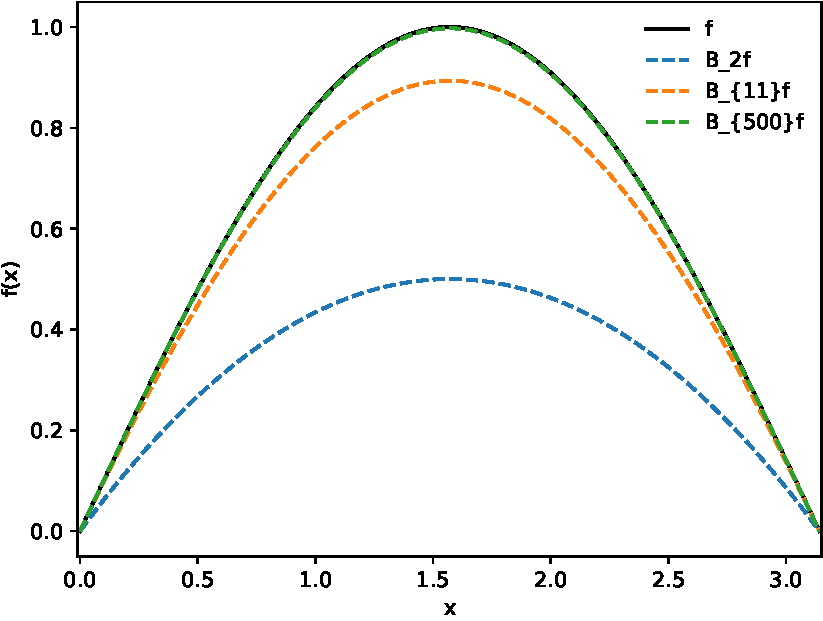
\includegraphics[width=0.68\textwidth]{scripts/approximation_sine.pdf}
		\caption{Approximation of $sin(x)$ by linear combination of Bernstein polynomials on $[a, b]$.}
		\label{fig:sine_approx}
	\end{figure}
\end{exmp}

